\section {The arduino}
\begin{frame} {Outline}
    \tableofcontents [current]
\end{frame}

% What is and why a micro-controller development board.
% It is a tool for making computers that can sense and control the physical world. 
\begin{frame} {Why a micro controller development board}
    \begin{itemize}
		\item to sense and control the physical world
		\item to develop interactive objects
		\item taking inputs from switches or sensors
		\item controlling lights, motors, …
		% \item then do many useful stuff based on that (or not)
    \end{itemize}
\end{frame}

% It's an open-source physical computing platform based on a simple 
% micro-controller board, the electronic behind the Arduino is quite simple, 
% and developing on it is very simple, it's C++ code with an development environment.

% There are many other micro-controllers and micro-controller platforms available 
% for physical computing. All of these tools take the messy details of 
% micro-controller programming and wrap it up in an easy-to-use package. 
% Arduino also simplifies the process of working with micro-controllers, but 
% it offers some advantage for teachers, students, and interested amateurs 
% over other systems:

\begin{frame}{Why Arduino ?}
	\begin{itemize}
		\item inexpensive (~ 22\$)
		% Inexpensive - Arduino boards are relatively inexpensive compared to other 
		% micro-controller platforms. The least expensive version of the Arduino 
		% module can be assembled by hand, and even the pre-assembled Arduino 
		% modules cost less than $50

		\item cross-platform (Windows, Mac OS X, Linux)
		% It's cross-platform, most micro-controller systems are limited to Windows.

		\item simple and don't require electronic skills
		% Simple, clear programming environment - The Arduino programming environment 
		% is easy-to-use for beginners, yet flexible enough for advanced users to take 
		% advantage of as well. 

		\item open source (software and hardware)
		% Open source and extensible hardware - 
		% The Arduino is based on Atmel's micro-controllers. 
		% The plans for the modules are published under a Creative Commons license.
	\end{itemize}
\end{frame}

% Most of the different kinds of arduino are composed by :
\begin{frame}{The micro controller development board}
    \begin{center}
		\includegraphics<1> [width=.9\textwidth,keepaspectratio] {img/arduino}
		\includegraphics<2> [width=.9\textwidth,keepaspectratio] {img/arduino_power_connector.jpg}
		% a power connector
		\includegraphics<3> [width=.9\textwidth,keepaspectratio] {img/arduino_usb.jpg}
		% an USB port (used as a power source and serial port)
		\includegraphics<4> [width=.9\textwidth,keepaspectratio] {img/arduino_reset_button.jpg}
		% a reset button
		\includegraphics<5> [width=.9\textwidth,keepaspectratio] {img/arduino_atmel_mc.jpg}
		% an ATmega micro controller
		\includegraphics<6> [width=.9\textwidth,keepaspectratio] {img/arduino_leds.jpg}
		% some leds (TX RX and pin 13 and power)
		\includegraphics<7> [width=.9\textwidth,keepaspectratio] {img/arduino_pins.jpg}
		% analog input pins (A0 to A5) some digital pins (0 to 13)
		\includegraphics<8> [width=.9\textwidth,keepaspectratio] {img/arduino_gnd_5v_3v3.jpg}
		% Ground, 5V and 3.3V pins
    \end{center}
\end{frame}

% we show the different components of the arduino board
\begin{frame}{And the other arduino boards}
	\begin{itemize}
		\item Due (ARM based)
		\item Lilypad (specially designed for wearables)
		\item … or do it yourself (not really difficult)
		% There is no real limit, you just do whatever you can do with the power supplied by arduino
	\end{itemize}
\end{frame}

\begin{frame}{The micro controller development board}
	\begin{columns} [c,onlytextwidth]
		\begin{column} [c] {.5\textwidth}
			\begin{center}
				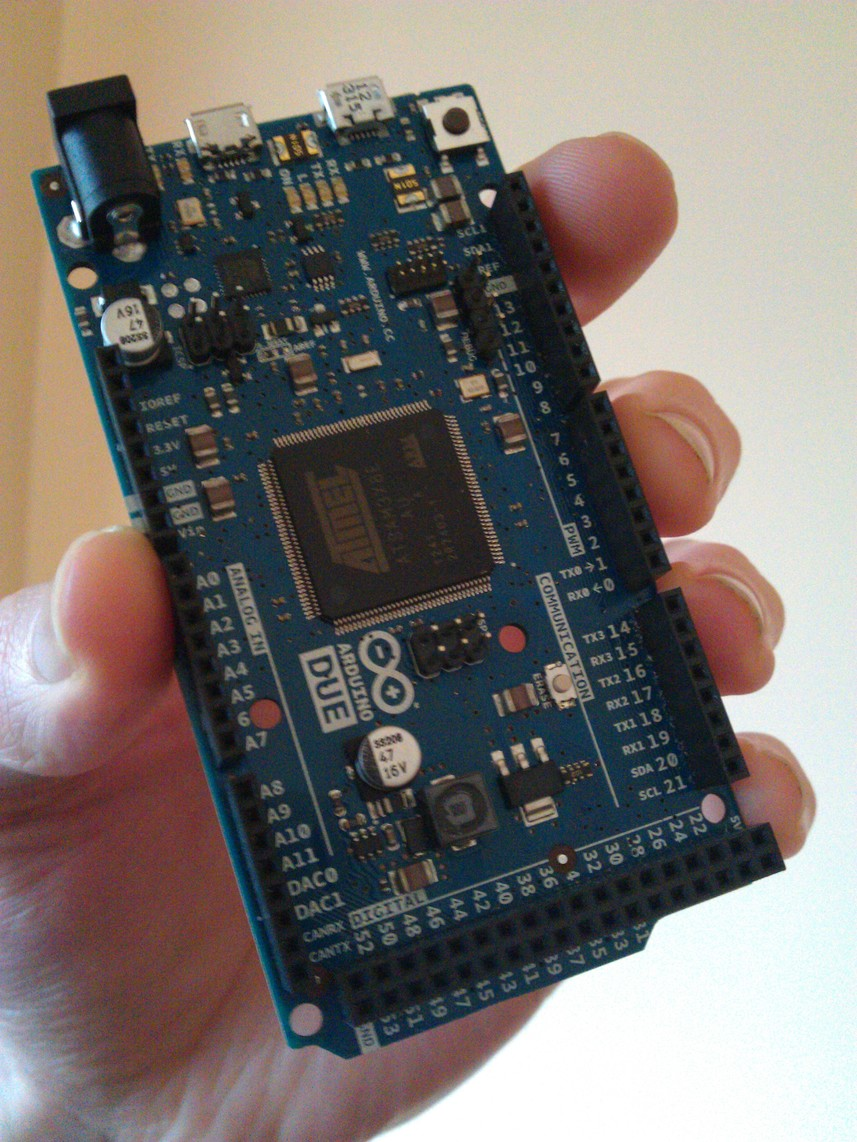
\includegraphics [width=.9\textwidth,keepaspectratio]{img/due}
			\end{center}
		\end{column}
		\begin{column} [c] {.5\textwidth}
			\begin{center}
				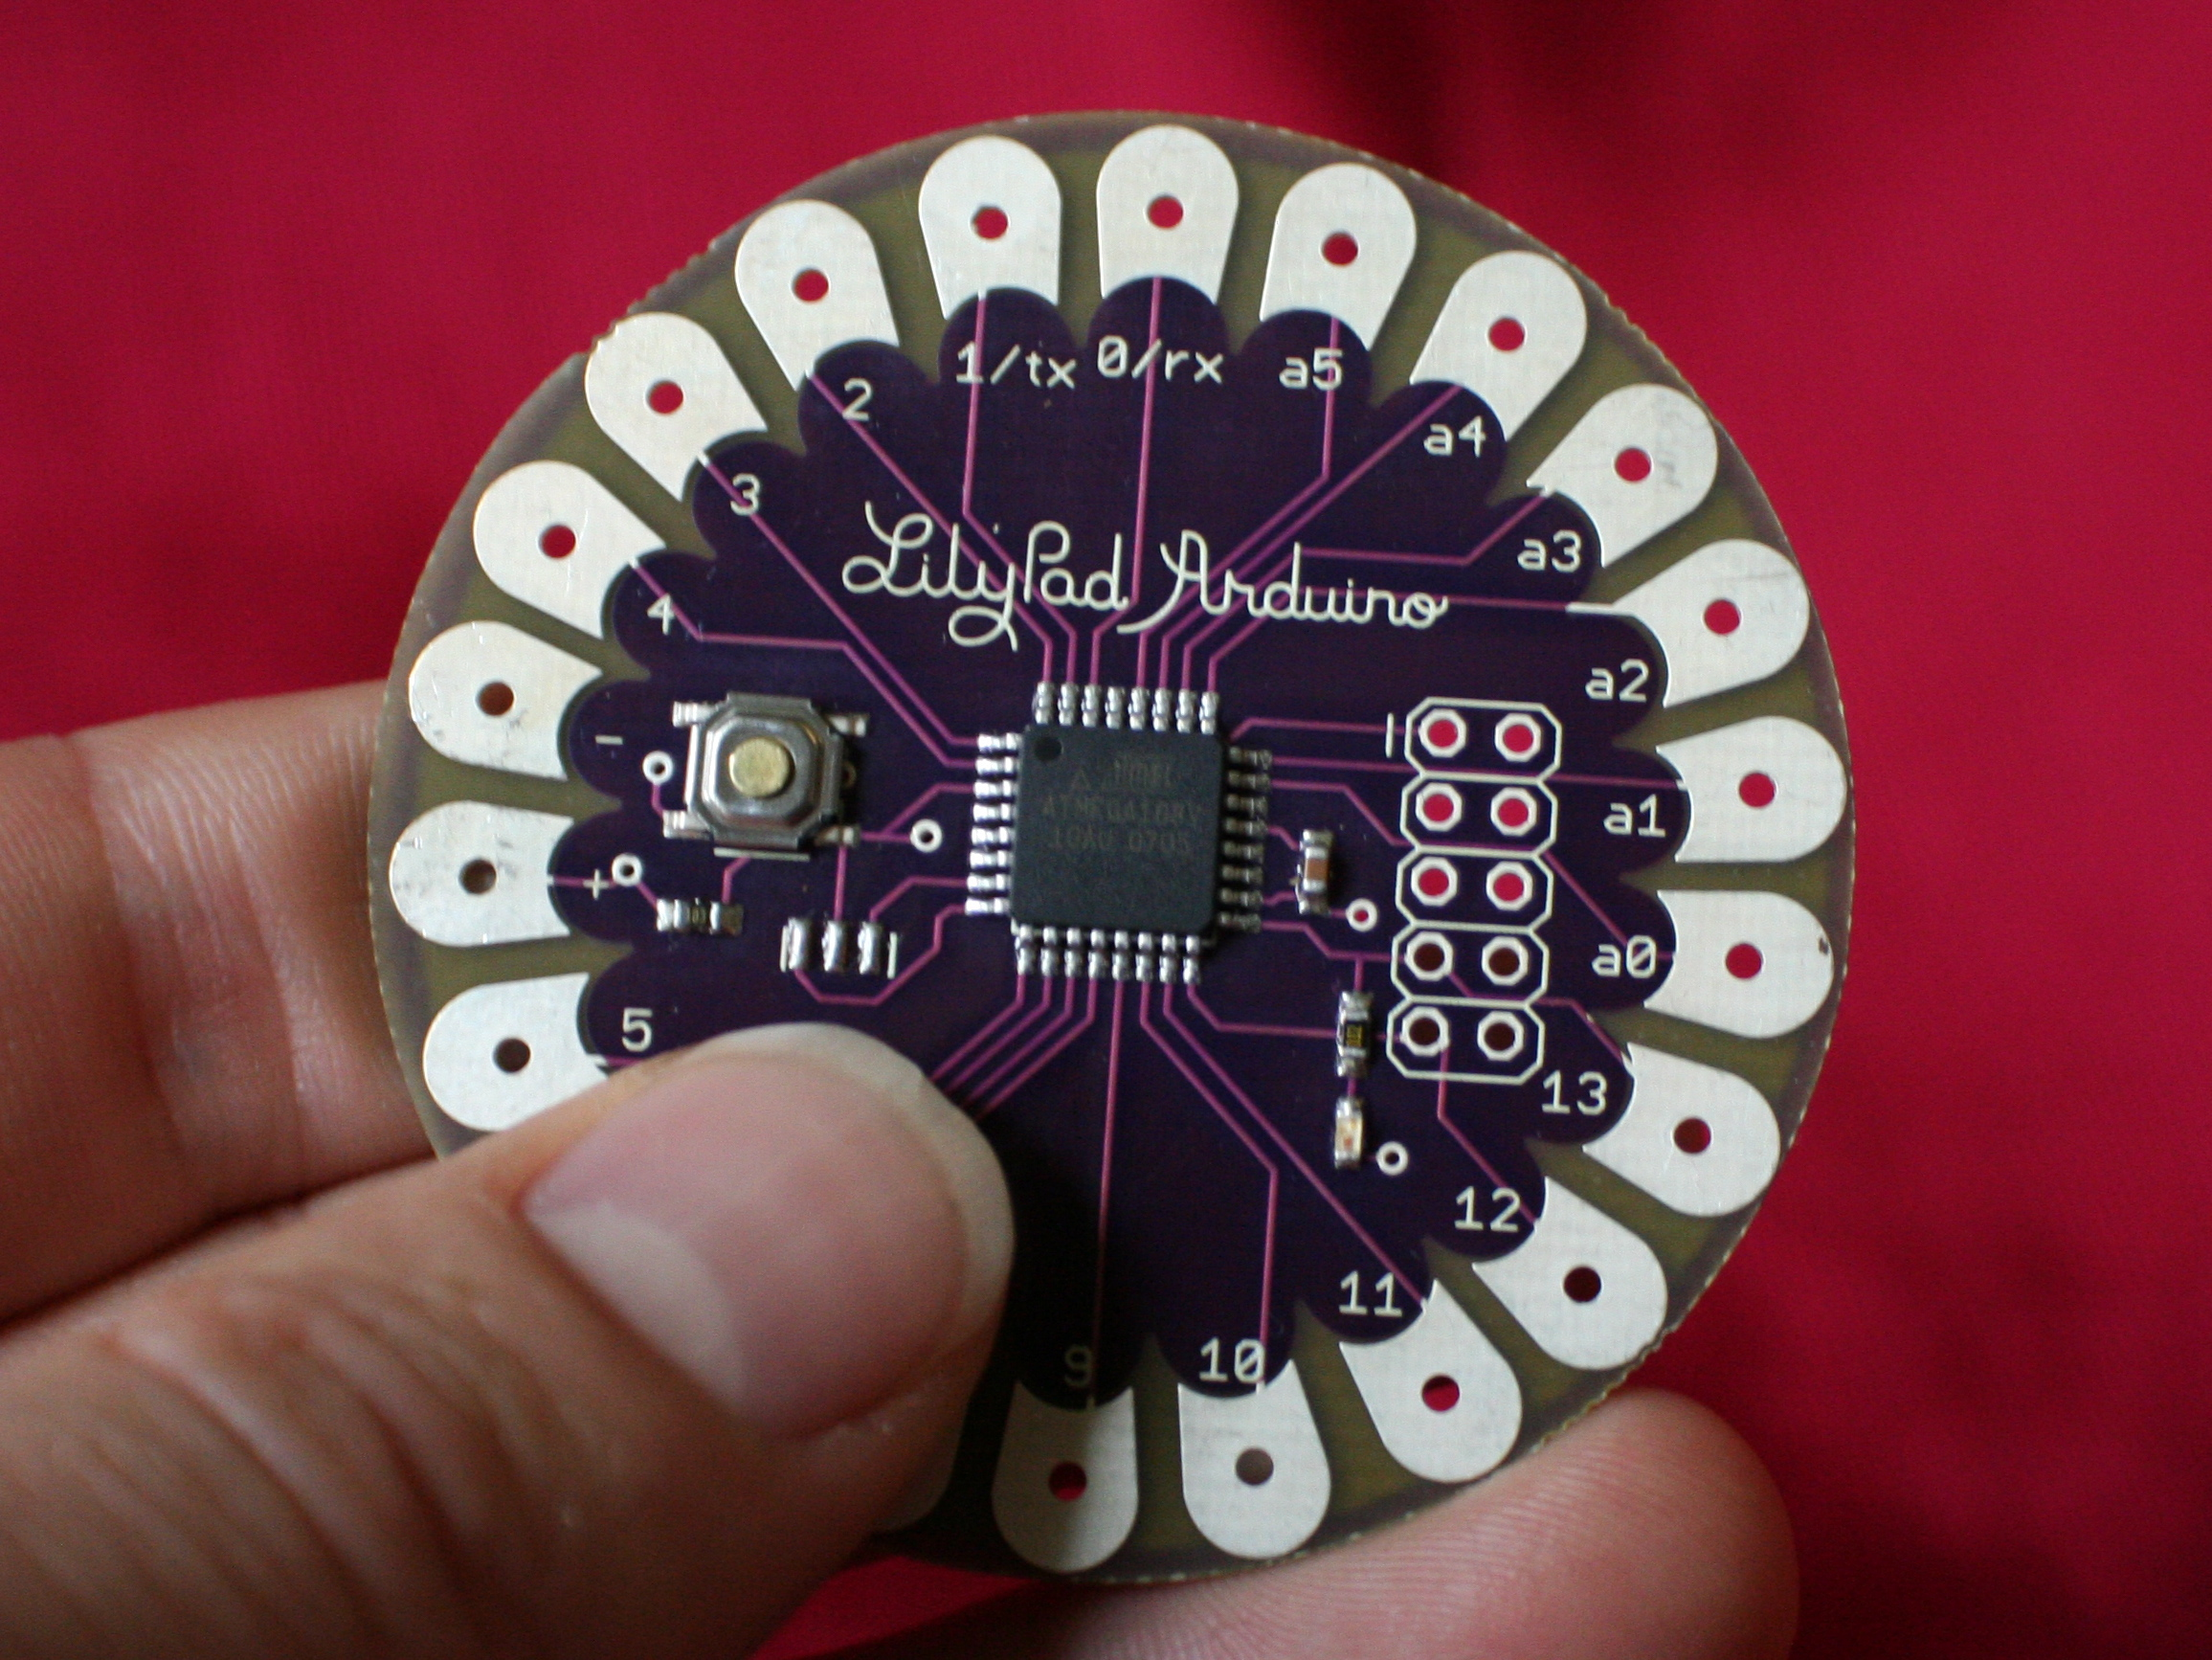
\includegraphics [width=.9\textwidth,keepaspectratio]{img/lilypad}
			\end{center}
		\end{column}
	\end{columns}
\end{frame}

\begin{frame}{How it works}
	\begin{itemize}
		\item powersource = running
	\end{itemize}
\end{frame}

\begin{frame}{How it works}
	\begin{center}
		\includegraphics<1> [width=1\textwidth,keepaspectratio] {pdf/arduino0.pdf}
		\includegraphics<2> [width=1\textwidth,keepaspectratio] {pdf/arduino1.pdf}
		\includegraphics<3> [width=1\textwidth,keepaspectratio] {pdf/arduino2.pdf}
	\end{center}
\end{frame}
% Arduino projects can be stand-alone, or they can communicate with software running on your computer.
